\documentclass{article}
\usepackage[utf8]{inputenc}
\usepackage{hyperref}
\usepackage[english]{babel}
\usepackage{latexsym,bm,amsmath,amssymb,graphicx,ctex,tikz,systeme,array, soul,scalerel,wrapfig,lipsum}
\newcommand*\circled[1]{\tikz[baseline=(char.base)]{
            \node[shape=circle,draw,inner sep=2pt] (char) {#1};}}
\usepackage{extarrows}% http://ctan.org/pkg/extarrows
\newcommand*{\vertbar}{\rule[-1ex]{0.5pt}{2.5ex}}
\newcommand*{\horzbar}{\rule[.5ex]{2.5ex}{0.5pt}}
\newcommand{\eqdef}{\xlongequal{\text{def}}}%
\usepackage{geometry}
 \geometry{
 a4paper,
 total={170mm,257mm},
 left=10mm,
 right=10mm,
 top=20mm,
 }
\usepackage{graphicx}
\usepackage{titling}
\usepackage{listings}
\usepackage{xcolor}
\usepackage[lighttt]{lmodern}
\definecolor{codegreen}{rgb}{0,0.6,0}
\definecolor{codegray}{rgb}{0.5,0.5,0.5}
\definecolor{codepurple}{rgb}{0.58,0,0.82}
\definecolor{backcolour}{rgb}{0.95,0.95,0.92}
\lstdefinestyle{mystyle}{
    backgroundcolor=\color{backcolour},   
    commentstyle=\color{codegreen},
    keywordstyle=\color{magenta},
    numberstyle=\tiny\color{codegray},
    stringstyle=\color{codepurple},
    basicstyle=\sffamily\large,
    breakatwhitespace=false,         
    breaklines=true,                 
    captionpos=b,                    
    keepspaces=true,                 
    numbers=left,                    
    numbersep=5pt,                  
    showspaces=false,                
    showstringspaces=false,
    showtabs=false,                  
    tabsize=2
}

\lstset{style=mystyle}
\newcommand{\subs}[1]{\subsection*{#1}}
\newcommand{\secs}[1]{\section*{#1}}
 
\usepackage{fancyhdr}
\fancypagestyle{plain}{%  the preset of fancyhdr 
    \fancyhf{} % clear all header and footer fields
    \fancyfoot[R]{Guyuan Xu\\224040074}
    \fancyfoot[L]{\thedate}
    \fancyhead[L]{MDS 6106 Optimization and Modeling}
    % \fancyhead[R]{\theauthor}
}
\makeatletter
\def\@maketitle{%
  \newpage
  \null
  \vskip 1em%
  \begin{center}%
  \let \footnote \thanks
    {\LARGE \@title \par}%
    \vskip 1em%
    %{\large \@date}%
  \end{center}%
  \par
  \vskip 1em}
\makeatother

% \usepackage{lipsum}  
% \usepackage{cmbright}



%======================================= document ======================================
%======================================= document ======================================
%======================================= document ======================================
\begin{document}

\title{\raggedright MDS 6106 Assignment 3}
%\author{Guyuan Xu \\224040074}
\date{Oct 28th, 2024}
\maketitle

\noindent\begin{tabular}{@{}ll}
   Guyuan Xu &\href{mailto:224040074@link.cuhk.edu.cn}{224040074} \\
    
%
\end{tabular}
%============ A3.1 ===============
\secs{A 3.1 Bisection and Golden Section Method}
\noindent\textcolor{blue}{Codes for implementation are attached at the end of this doc}\\
\begin{figure}[h]
    \centering
    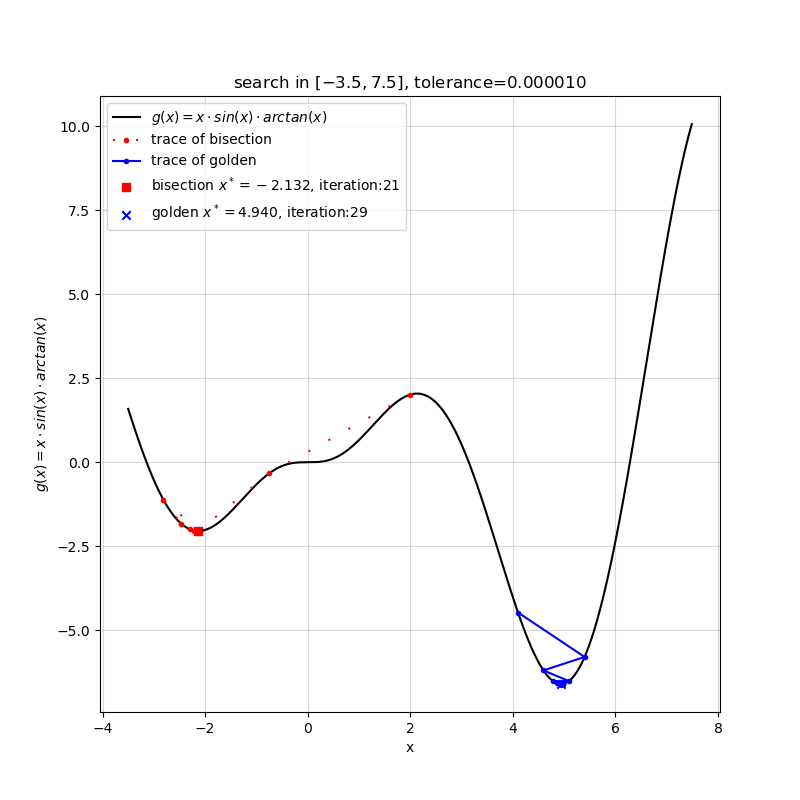
\includegraphics[scale = 0.8]{left_-3.5_right_7.5.png}
    \caption{search in $[-3.5,7.5]$}
\end{figure}
By implementing the given settings, we find that Bisection and Golden section covnerge at different points, and it takes 21 iteration for Bisection to converge by the tolerance requirement while 29 iteration for Golden section.\\\vspace{5mm}

We then set the initial setting different from given and search in $[-3,7.5]$ (check results below) :
\begin{figure}[th]
    \centering
    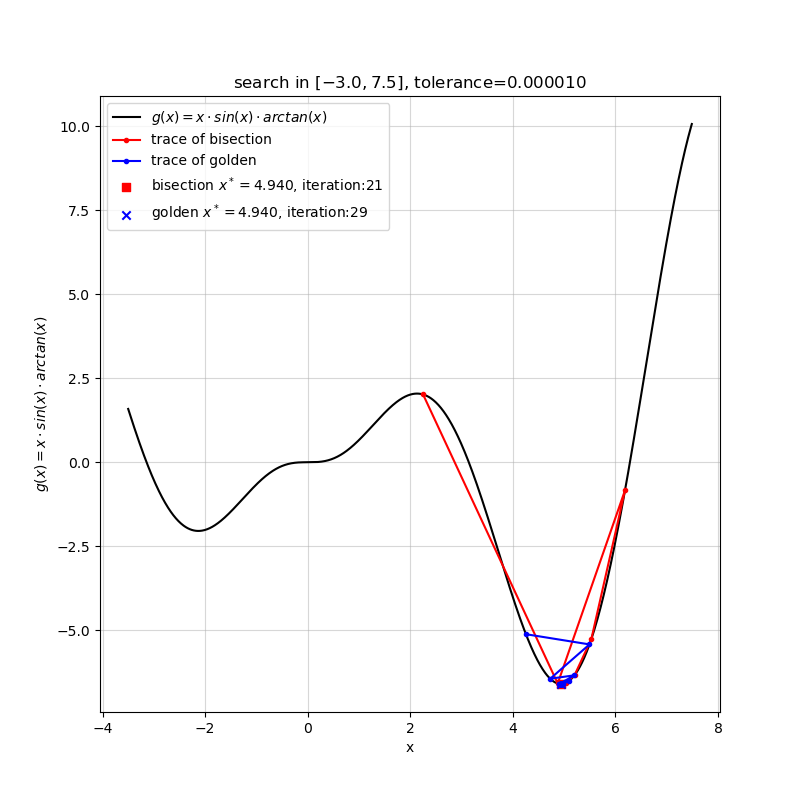
\includegraphics[scale = 0.8]{left_-3.0_right_7.5.png}
    \caption{search in $[-3,7.5]$}
\end{figure}
We find that both searching methods converge at same point, the iterations they take are the same as before: 21 for bisection and 29 for golden section. \textbf{This may tell us the convergence depends on the inital settings.}


%============ A3.2 ================
\secs{A 3.2 Descent Directions}
\subs{a)}
\[
\nabla f(x) = \begin{pmatrix}
    \frac{\partial f}{\partial x_1}\\
    \frac{\partial f}{\partial x_1}\\
    \vdots \\
    \frac{\partial f}{\partial x_n}
\end{pmatrix},\;\;
e_j = \begin{pmatrix}
    0\\
    \vdots\\
    0\\
    1\\
    0\\
    \vdots\\
    0
\end{pmatrix} \leftarrow\;\text{j-th item, then }
d = -\frac{\partial f}{\partial x_j} e_j = \begin{pmatrix}
    0\\
    \vdots\\
    0\\
    -\frac{\partial f}{\partial x_j}\\
    0\\
    \vdots\\
    0
\end{pmatrix}
\]
so
\[
\nabla f(x)^T d = \left[\frac{\partial f}{\partial x_1},...,\frac{\partial f}{\partial x_n}\right]\cdot \begin{pmatrix}
0\\
\vdots\\
0\\
-\frac{\partial f}{\partial x_j}\\
0\\
\vdots\\
0
\end{pmatrix} = -\left[\frac{\partial f}{\partial x_j}\right]^2 < 0 \text{ since }\nabla f(x)\neq 0 \text{ and } \left|\frac{\partial f}{\partial x_j}\right| \text{ is the largest one}
\]
\textcolor{red}{thus $\nabla f(x)^T d <0$ means $d$ is a descent direction.}


%============= b) ===================
\subs{b)}

\[
D^{-1}=\begin{pmatrix}
    \frac{1}{\delta_1} & 0 & ... & 0\\
 0 & \frac{1}{\delta_2} & ... & 0\\
 \vdots & \vdots & ... & 0\\
  0 & 0 & ... &\frac{1}{\delta_n}
\end{pmatrix} = diag\{\frac{1}{\delta_1},...,\frac{1}{\delta_n}\},\; \delta_i > 0,\;\forall i
\]
then\[
    \nabla f(x)^T d  = -1*\left[\frac{\partial f}{\partial x_1},...,\frac{\partial f}{\partial x_n}\right]\cdot 
    \begin{pmatrix}
        \frac{1}{\delta_1} & 0 & ... & 0\\
     0 & \frac{1}{\delta_2} & ... & 0\\
     \vdots & \vdots & ... & 0\\
      0 & 0 & ... &\frac{1}{\delta_n}
    \end{pmatrix}\cdot
    \begin{pmatrix}
        \frac{\partial f}{\partial x_1}\\
        \frac{\partial f}{\partial x_1}\\
        \vdots \\
        \frac{\partial f}{\partial x_n}
    \end{pmatrix} = -\sum_{i=1}^{n}\frac{1}{\delta_i} \left[\frac{\partial f}{\partial x_1}\right]^2
\]
since $\delta_i>0$ for all i, $\displaystyle \frac{1}{\delta_j} \left[\frac{\partial f}{\partial x_j}\right]^2 \geq 0, \forall i$.  On the other hand $\nabla f(x) \neq 0$, then there exists $j$, such that $\frac{1}{\delta_j} \left[\frac{\partial f}{\partial x_j}\right]^2 >0$
hence 
\[
    \nabla f(x)^T d = -\sum_{i=1}^{n}\frac{1}{\delta_i} \left[\frac{\partial f}{\partial x_1}\right]^2 \leq 
    -\frac{1}{\delta_j} \left[\frac{\partial f}{\partial x_j}\right]^2 < 0
\]
\textcolor{red}{thus $\nabla f(x)^T d <0$ means $d$ is a descent direction.}



%============= A3.3 ==================
\secs{A3.3 Lipschitz Continuity}
%============== a) =================
\subs{a)}
\textbf{In this problem, we take 1-norm with respect to both matrix and vector.}
\[
\nabla f_1(x) = \begin{pmatrix}
    3x_1+2x_2\\
    2x_1\\
    -x_3^2
\end{pmatrix},\;\;
\nabla^2 f_1(x) = \begin{pmatrix}
    3 & 2 & 0\\
    2 & 0 & 0\\
    0 & 0 & -2x_3
\end{pmatrix}
\]
then $\|\nabla^2 f_1(x)\|_1$ is the max of the absolute value of the sum of its column, that is $\|\nabla^2 f_1(x)\|_1 = \max \{5,2,|2x_3|\}$, this is obsviously unbounded, since $|2x_3|$ can be infinitly large when $x_3 \rightarrow +\infty$, by the equivalence of norm boundedness we can conclude that \textcolor{red}{$f_1(x)$ is not Lipschitz continuous because its Hessian is unbounded}.


%============= b) ==================
\subs{b)}
\textbf{In this problem, we take 2-norm with respect to both matrix and vector.}
\[
\nabla f_2(x) = \begin{pmatrix}
    \frac{x_1}{\sqrt{1+x_1^2+x_2^2}}\\
    \frac{x_2}{\sqrt{1+x_1^2+x_2^2}}
\end{pmatrix} \;\;\circled{1}\text{, we then let }g(x)=\frac{1}{\sqrt{1+x_1^2+x_2^2}} = \frac{1}{\sqrt{1+\|x\|_2^2}}, x\in \mathbb{R}^2
\]
then the differential of $g(x)$ with respect to vector $x$:
\[
x\in \mathbb{R}^2:g^\prime (x)=-\frac{1}{2}\left[\frac{1}{\sqrt{1+\|x\|_2^2}}\right]^3
\]
then, the gradient \circled{1} can be rewriten as:
\[
\nabla f_2(x)= 
\begin{pmatrix}
    x_1 g(x)\\
    x_2 g(x)
\end{pmatrix}
\]
we then proceed to the hessian:
\[
\nabla^2 f_2(x) = \begin{pmatrix}
    g(x)+2 g^\prime (x) x_1^2 & 2 g^\prime (x) x_1 x_2\\
    2 g^\prime (x) x_1 x_2 & g(x)+2g^\prime (x) x_2^2
\end{pmatrix}\;\;\circled{2}
\]
Notice that the Hessian is a real symmetric 2x2 martrix, the 2-norm of it equal to the maximum of the abosolute value of its eigenvalues, that is
\[
\|\nabla^2 f_2(x)\|_2 =\|\lambda\|_{\infty} =\max{\{|\lambda_1|,|\lambda_2|\}}
\]
for simplification, denote \[
\nabla^2 f_x(x) = \begin{pmatrix}
    a & b\\
    b & c
\end{pmatrix}\text{, where }a = g(x)+2 g^\prime (x) x_1^2,\; b = 2 g^\prime (x) x_1 x_2,\; c = g(x)+2g^\prime (x) x_2^2
\]
the eigen-polynomial
\[
\begin{vmatrix}
    a-\lambda & b\\
    b & c-\lambda
\end{vmatrix} = 0 = \lambda^2-(a+c)\lambda +ac-b^2 \Rightarrow
\lambda_1,\;\lambda_2 = \frac{a+c\pm \sqrt{(a+c)^2+4(b^2-ac)}}{2} \;\;\circled{3}
\]
notice that
\[
    (a+c)^2+4(b^2-ac) =a^2+c^2+4b^2-2ac = (a-c)^2+4b^2 =\left[
        2g^\prime (x) x_1^2-2g^\prime (x) x_2^2
    \right]^2+4 \left[
        2g^\prime(x)^2x_1^2 x_2^2
    \right] = 4 \left[
        g^\prime (x) x_1^2+g^\prime (x) x_2^2
    \right]^2 \;\;\circled{4}
\]
and \[
    g^\prime (x)=-\frac{1}{2}\left[\frac{1}{\sqrt{1+\|x\|_2^2}}\right]^3 < 0
\]
\circled{4} plug into \circled{3} we have 
\[
\circled{3} = \frac{2g(x)+2g^\prime (x)\left[x_1^2+x_2^2\right]\pm 2g^\prime (x)\left[x_1^2+x_2^2\right]}{2}\] 

\[\Rightarrow \lambda_1 = g(x) =  \frac{1}{\sqrt{1+\|x\|_2^2}},\; \lambda_2 = g(x)+2g^\prime (x)\left[x_1^2+x_2^2\right] =\frac{1}{\sqrt{1+\|x\|_2^2}} -\frac{1}{2}\left[\frac{1}{\sqrt{1+\|x\|_2^2}}\right]^3 \cdot 2\|x\|_2^2 = \frac{1}{\sqrt{1+\|x\|_2^2}}\frac{1}{1+\|x\|_2^2}
\]
since $\displaystyle \left|\frac{1}{1+\|x\|_2^2}\right|\leq 1$, we always have
\[
|\lambda_2| = \left|\frac{1}{\sqrt{1+\|x\|_2^2}}\frac{1}{1+\|x\|_2^2}\right| \leq \left|\frac{1}{\sqrt{1+\|x\|_2^2}}\right| = |\lambda_1|
\]
hence
\[
    \|\nabla^2 f_2(x)\|_2 =\|\lambda\|_{\infty} =\max{\{|\lambda_1|,|\lambda_2|\}} = |\lambda_1| = \left|\frac{1}{\sqrt{1+\|x\|_2^2}}\right|
\]
when $\|x\|=0\iff x_1=x_2=0$, $|\lambda_1|$ hits the global maximum $1$, meaning $\|\nabla^2 f_2(x)\|_2 \leq 1$, then we can conclude that \textcolor{red}{ $f_2(x)$ is Lipschitz continuous in $\mathbb{R}^2$, if we take the 2-norm as the matrix and vector norm, the Lipschitz constant is $1$.}


%============= c) ===============
\subs{c)}
\textbf{we take 2-norm for both matrix and vector like part b), }$f_3(x)$ looks nice, so we directly calculate its hessian
\[
\nabla f_3(x)=\begin{pmatrix}\displaystyle
    \frac{2x_1}{1+x_1^2}\\
    \displaystyle \frac{2x_2}{1+x_2^2}
\end{pmatrix},\;\;
\nabla^2 f_3(x) = \begin{pmatrix}\displaystyle
    \frac{2(1-x_1^2)}{(1+x_1^2)^2} & 0\\
    \displaystyle 0 &\displaystyle  \frac{2(1-x_2^2)}{(1+x_2^2)^2}
\end{pmatrix}
\]
we can see that $\nabla^2 f_3(x)$ is a diagonal matrix (and is symmetric obviously) the eigen values are its diagonal elements: 
\[
\lambda_1 = \frac{2(1-x_1^2)}{(1+x_1^2)^2},\; \lambda_2 = \frac{2(1-x_2^2)}{(1+x_2^2)^2}
\]
denote $\displaystyle g(t) = \frac{2(1-t)}{(1+t)^2},\; t \geq 0$\begin{itemize}
    \item when $0 \leq t \leq 1$, $g(t)\geq 0$ ,and the numerator $2(1-t) \searrow  $ as $t \nearrow$, while the denominator $(1+t)^2 \nearrow $ as $t \nearrow$, so $g(t)$ is monotonously decreasing in $[0,1]$, \textcolor{red}{so the maximum of $g(x)$ in [0,1] is $g(0) = 2$ $\Rightarrow 0\leq |g(t)| = g(t)\leq 2,\; 0\leq t \leq 1$}
    \item when $t\geq 1$, $g(t)\leq 0$, $\displaystyle g^\prime (t) = \frac{2(t-3)(t+1)}{(1+t)^4}$, then $g^\prime (t)=0, \text{when }t=3$, so (by the sign of $g^\prime (t), t \geq 1$) $g(t)$ hits its minimum $g(3) = -\frac{1}{4}$, when $t=3$, so $-\frac{1}{4}\leq g(t) \leq 0 \Rightarrow 0 \leq|g(t)|\leq \frac{1}{4}, t\geq 1$
\end{itemize}
then we can conclude that $g(x)$ hits maximum at $t=0$, minimum at $t=3$ when $t \in [0,+\infty)$, notice that $\displaystyle \lambda = g(x^2)$, since $x^2\geq 0$, we can conclude that the maximum of the absolute value of eigenvalues $\max \{|\lambda|\} = \underset{x\in \mathbb{R}^1}{\max}|g(x^2)| = g(0) = 2$
then $\|\nabla^2 f_3(x)\|_2 = \max{\{|\lambda_1|,|\lambda_2|\}} = 2$, when $x_1\text{ or } x_2 = 0$ (remember x = $\begin{pmatrix}
    x_1\\
    x_2
\end{pmatrix}$)\\
from the above reasoning we can conclude that \textcolor{red}{$f_3(x)$ is Lipschitz continuous since its Hessian is bounded by 2 if we take 2-norm of matrix, and the Lipschitz constant is $2$}.


\begin{center}
    \begin{tabular}{|c|cccc|} 
        \hline
        Methods & $x_0$ & iteration & limit point $x^*$ & $\|x_0-x^*\|_2$ \\
        \hline
        &(-0.50,1.00) & 13 & (2.00,-0.00) & 2.69 \\ % backtrack
        &(-0.50,0.50) & 325 & (-0.00,1.00) & 0.71 \\ % backtrack
        Back Tracking&(-0.25,-0.50) & 467 & (-0.00,-1.00) & 0.56 \\ % backtrack
        &(0.50,-0.50) & 12 & (2.00,0.00) & 1.58 \\ % backtrack
        &(0.50,1.00) & 10 & (2.00,-0.00) & 1.80 \\ % backtrack
        \hline
        \hline
        &(-0.50,1.00) & 295 & (-0.00,1.00) & 0.50 \\ % exactlineS
        &(-0.50,0.50) & 296 & (-0.00,1.00) & 0.71 \\ % exactlineS
        Exact Line Search&(-0.25,-0.50) & 375 & (-0.00,-1.00) & 0.56 \\ % exactlineS
        &(0.50,-0.50) & 9 & (2.00,0.00) & 1.58 \\ % exactlineS
        &(0.50,1.00) & 6 & (2.00,0.00) & 1.80 \\ % exactlineS
        \hline
        \hline
        &(-0.50,1.00) & 47 & (2.00,0.00) & 2.69 \\ % diminishing
        &(-0.50,0.50) & 8523 & (-0.00,1.00) & 0.71 \\ % diminishing
        Diminishing Stepsize&(-0.25,-0.50) & 8501 & (-0.00,-1.00) & 0.56 \\ % diminishing
        &(0.50,-0.50) & 47 & (2.00,-0.00) & 1.58 \\ % diminishing
        &(0.50,1.00) & 47 & (2.00,0.00) & 1.80 \\ % diminishing
      \hline
    \end{tabular} 
\end{center}

\begin{figure}[h]
    \centering
    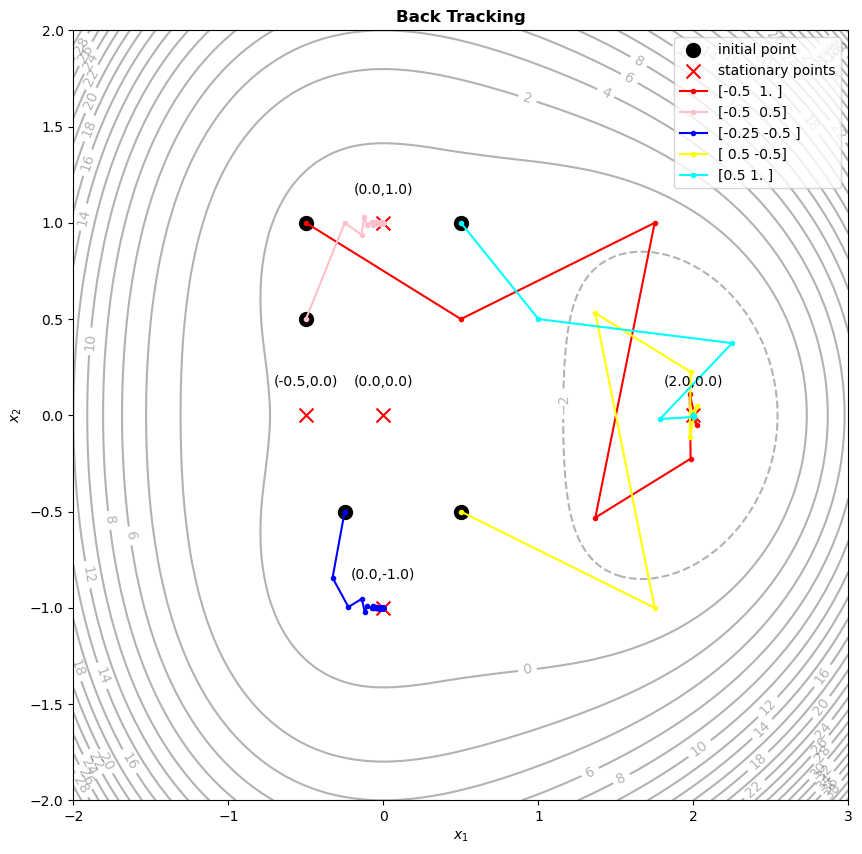
\includegraphics[scale = 0.8]{Back Tracking.png}
\end{figure}













\end{document}


